% !TXS template
\documentclass[french]{scrartcl}
\usepackage[T1]{fontenc}
\usepackage[utf8]{inputenc}
\usepackage{lmodern}
\usepackage[a4paper]{geometry}
\usepackage{babel}
\usepackage{graphicx}
\usepackage[]{babel}
\usepackage{multicol}
\usepackage{multicol}
\usepackage{amsmath}
\usepackage{amsthm}
\usepackage{amsfonts}
\usepackage{siunitx}
\usepackage{braket}
\usepackage{booktabs}
\usepackage{amssymb}
\usepackage{makeidx}
\usepackage{graphicx}
\usepackage[export]{adjustbox}
\usepackage{scalerel}
\usepackage{mathrsfs}
\usepackage{tikz}
\usepackage{url}
\author{Manuel Luci, Andrea Dell'Abate}
\title{CMPEDA Project: Lending Club loan data prediction}
\date{}
\subtitle{A Finance Predictive Model based on DNN and XGboost}
\begin{document}
\maketitle
\section{Introducion}
LendingClub is a US peer-to-peer lending company which specialises in lending various types of loans to urban customers.\\
When the company receives a loan application, we have to make a decision based on the applicant’s profile. \\
Two types of risks are associated with the bank's decision:
\begin{itemize}
	\item if the applicant is likely to repay the loan, then not approving it results in a loss of business to the company;
	
	\item if the applicant is not likely to repay the loan, i.e. he/she is likely to
	default, then approving it may lead to a financial loss for the company.
\end{itemize}
Our aim is to develop the best supervised machine learning model capable to identify which borrowers will payoff their loans.\\
We’ll try to do this binary classification task using Deep Neural Network and X-G
boost models.\\
Link dataset:\url{https://www.kaggle.com/code/faressayah/lending-club-loan-defaulters-prediction/data?select=lending_club_loan_two.csv}
\section{Preprocessing (module: data\_analysis )}
We divided the preprocessing part into two phases: 
\begin{itemize}
	\item In the first one we developed the statistical part of the dataset analyzing how all the features were distributed and how they were correlated with each other.
	\item In the second part we modified the dataset for our purposes: the missing values were treated (eliminating or replacing them as appropriate), we eliminated the variables that were highly correlated with each other and  we chose those that were most useful for our machine learning task.\\
	Finally we replaced all categorical variables with numeric ones and we performed the one hot encoder by means of the dummy module (dummy data).\\
\end{itemize}
Below we report some usefull graphs for our analysis:
	\begin{figure}[h!]
		\centering
		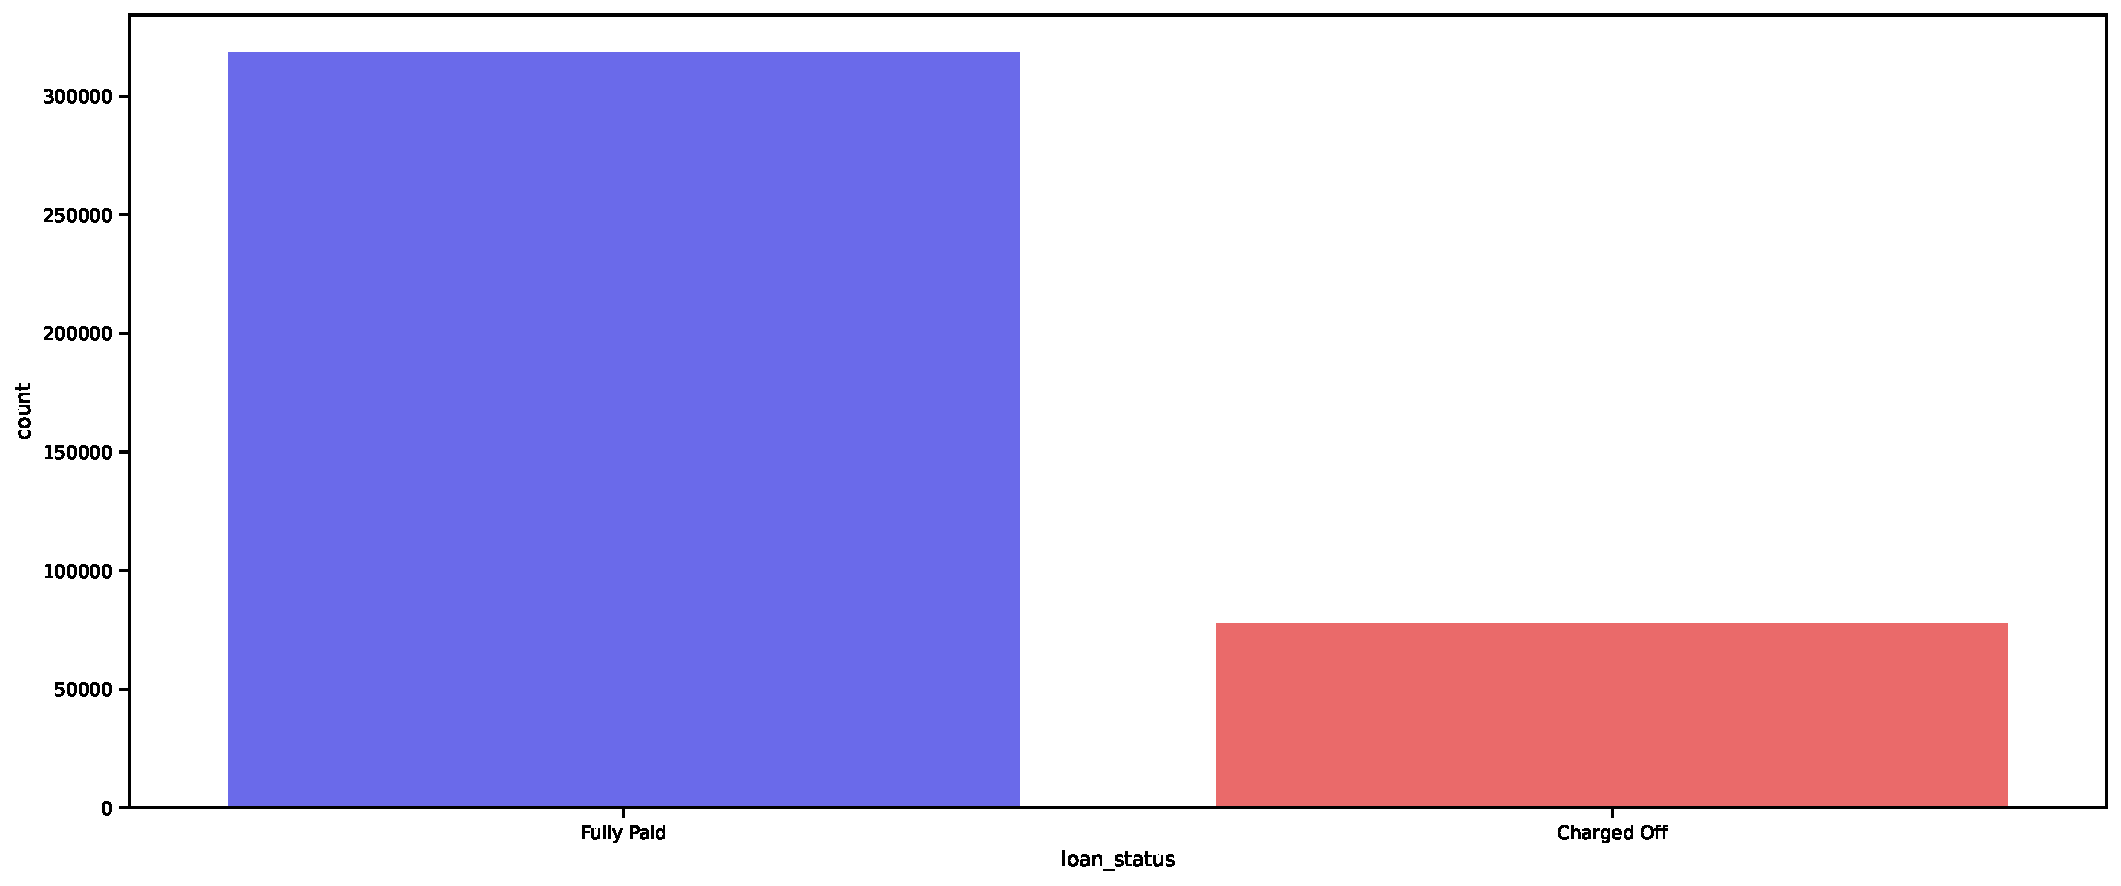
\includegraphics[scale=0.3]{figures/(1)pf_vs_co.pdf}
		\caption{loan\_status distribution, we can see that our database is strictly unbalanced}
	\end{figure}
	\begin{figure}[h!]
	    \centering
	    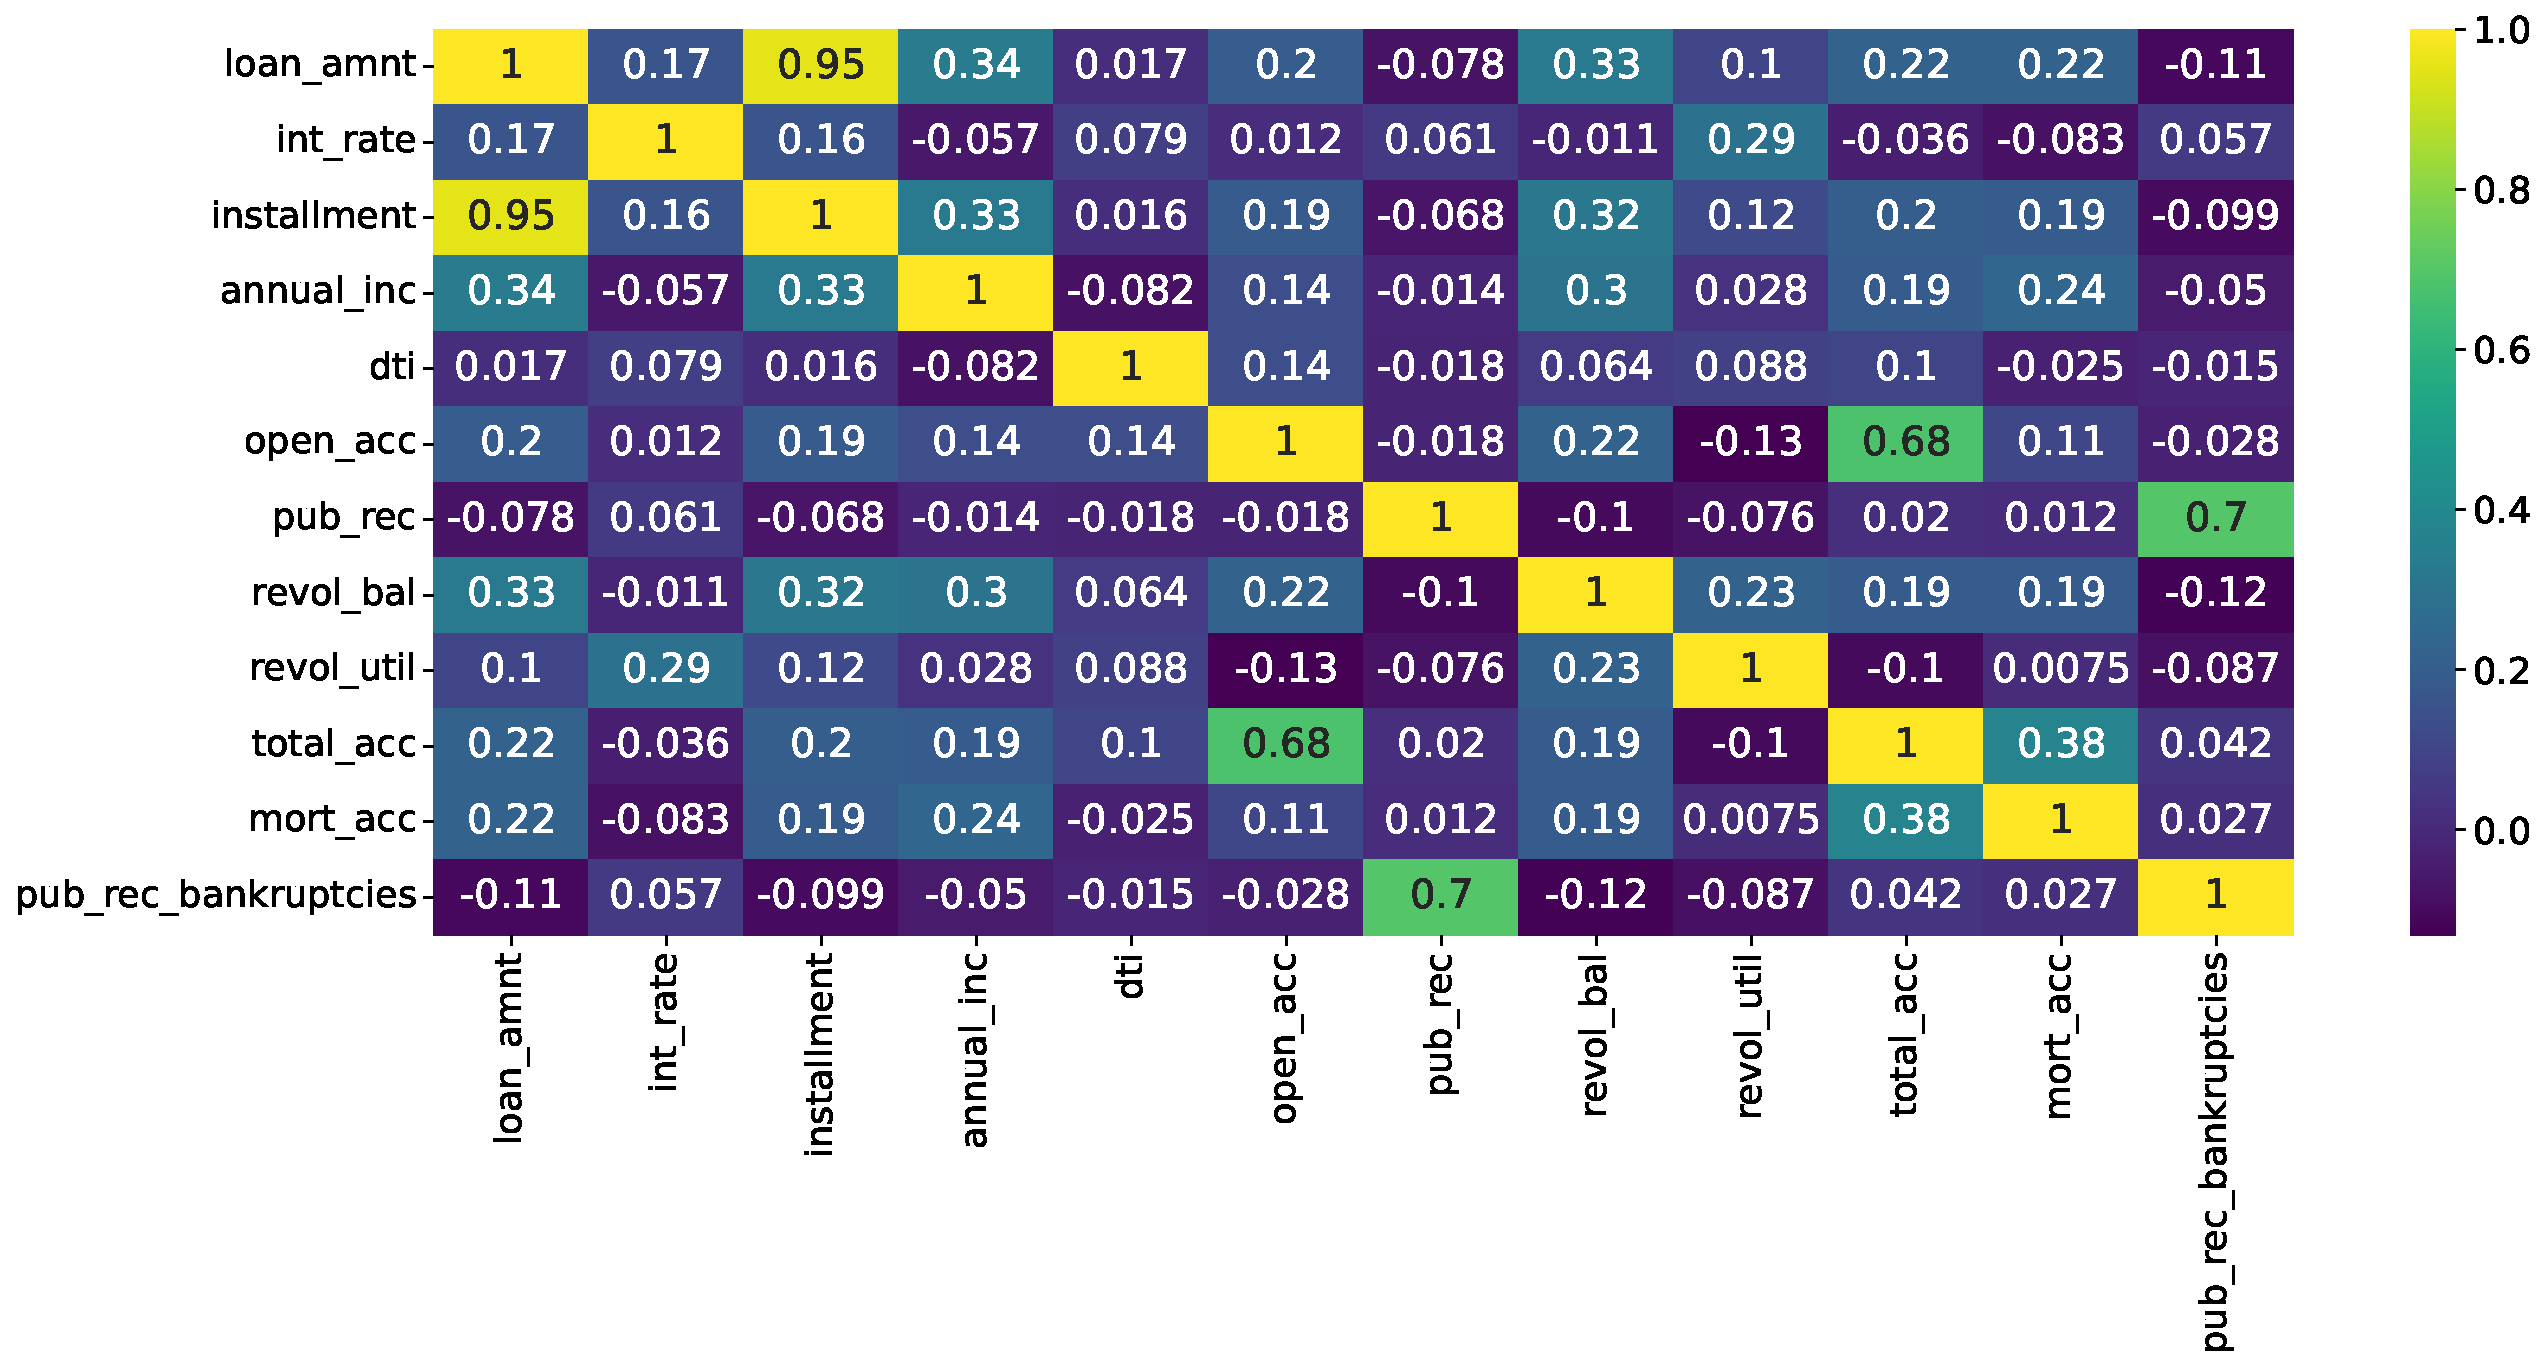
\includegraphics[scale=0.3]{figures/(2)corr_matrix}
	    \caption{Correlation matrix}
	\end{figure}
	\begin{figure}[h!]
	\centering
	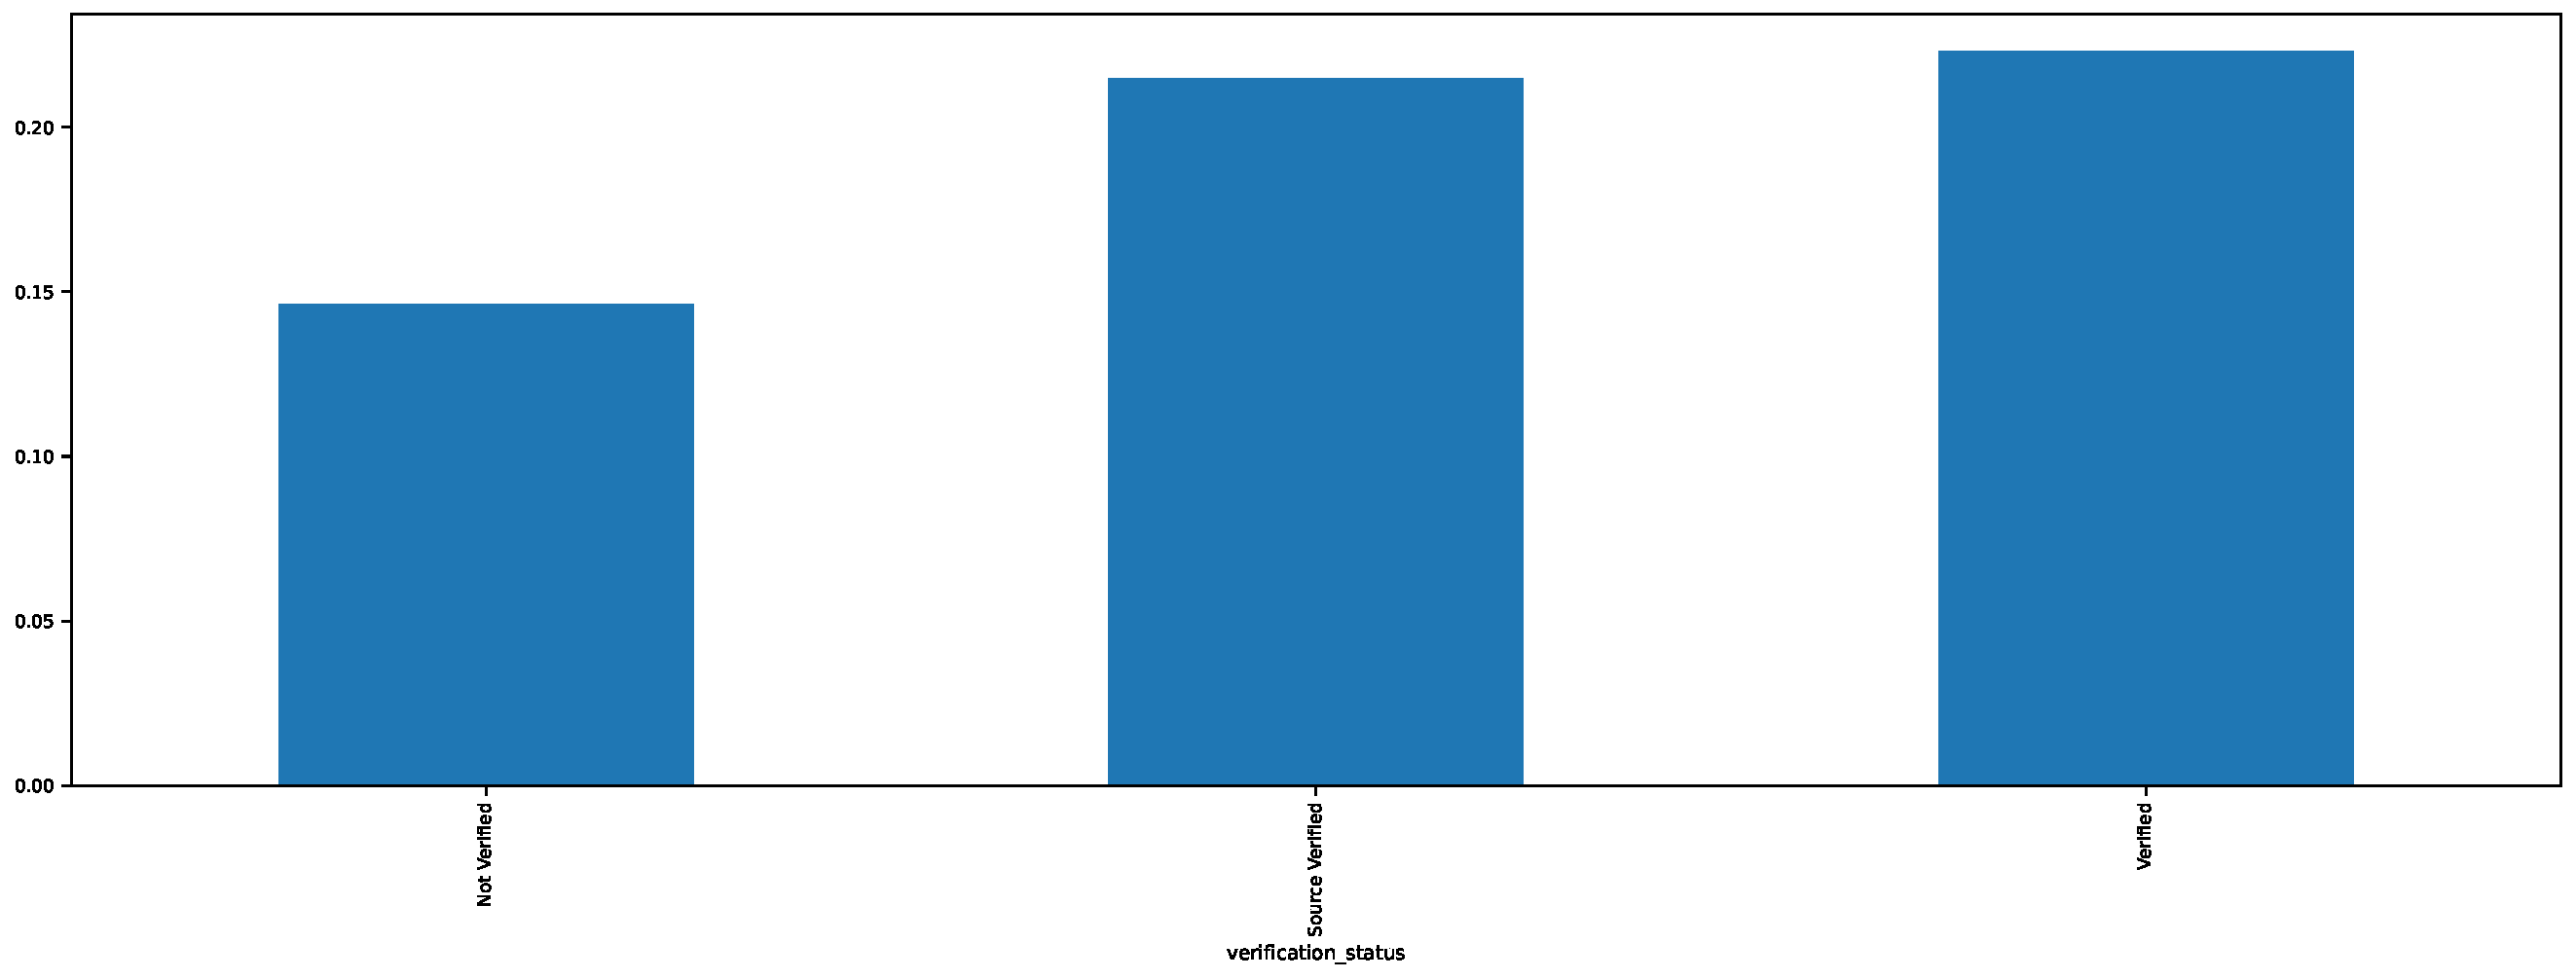
\includegraphics[scale=0.3]{figures/(3)verification_status_bar.pdf}
	\caption{barplot verification\_status distribution}
    \end{figure}
	\begin{figure}[h!]
	\centering
	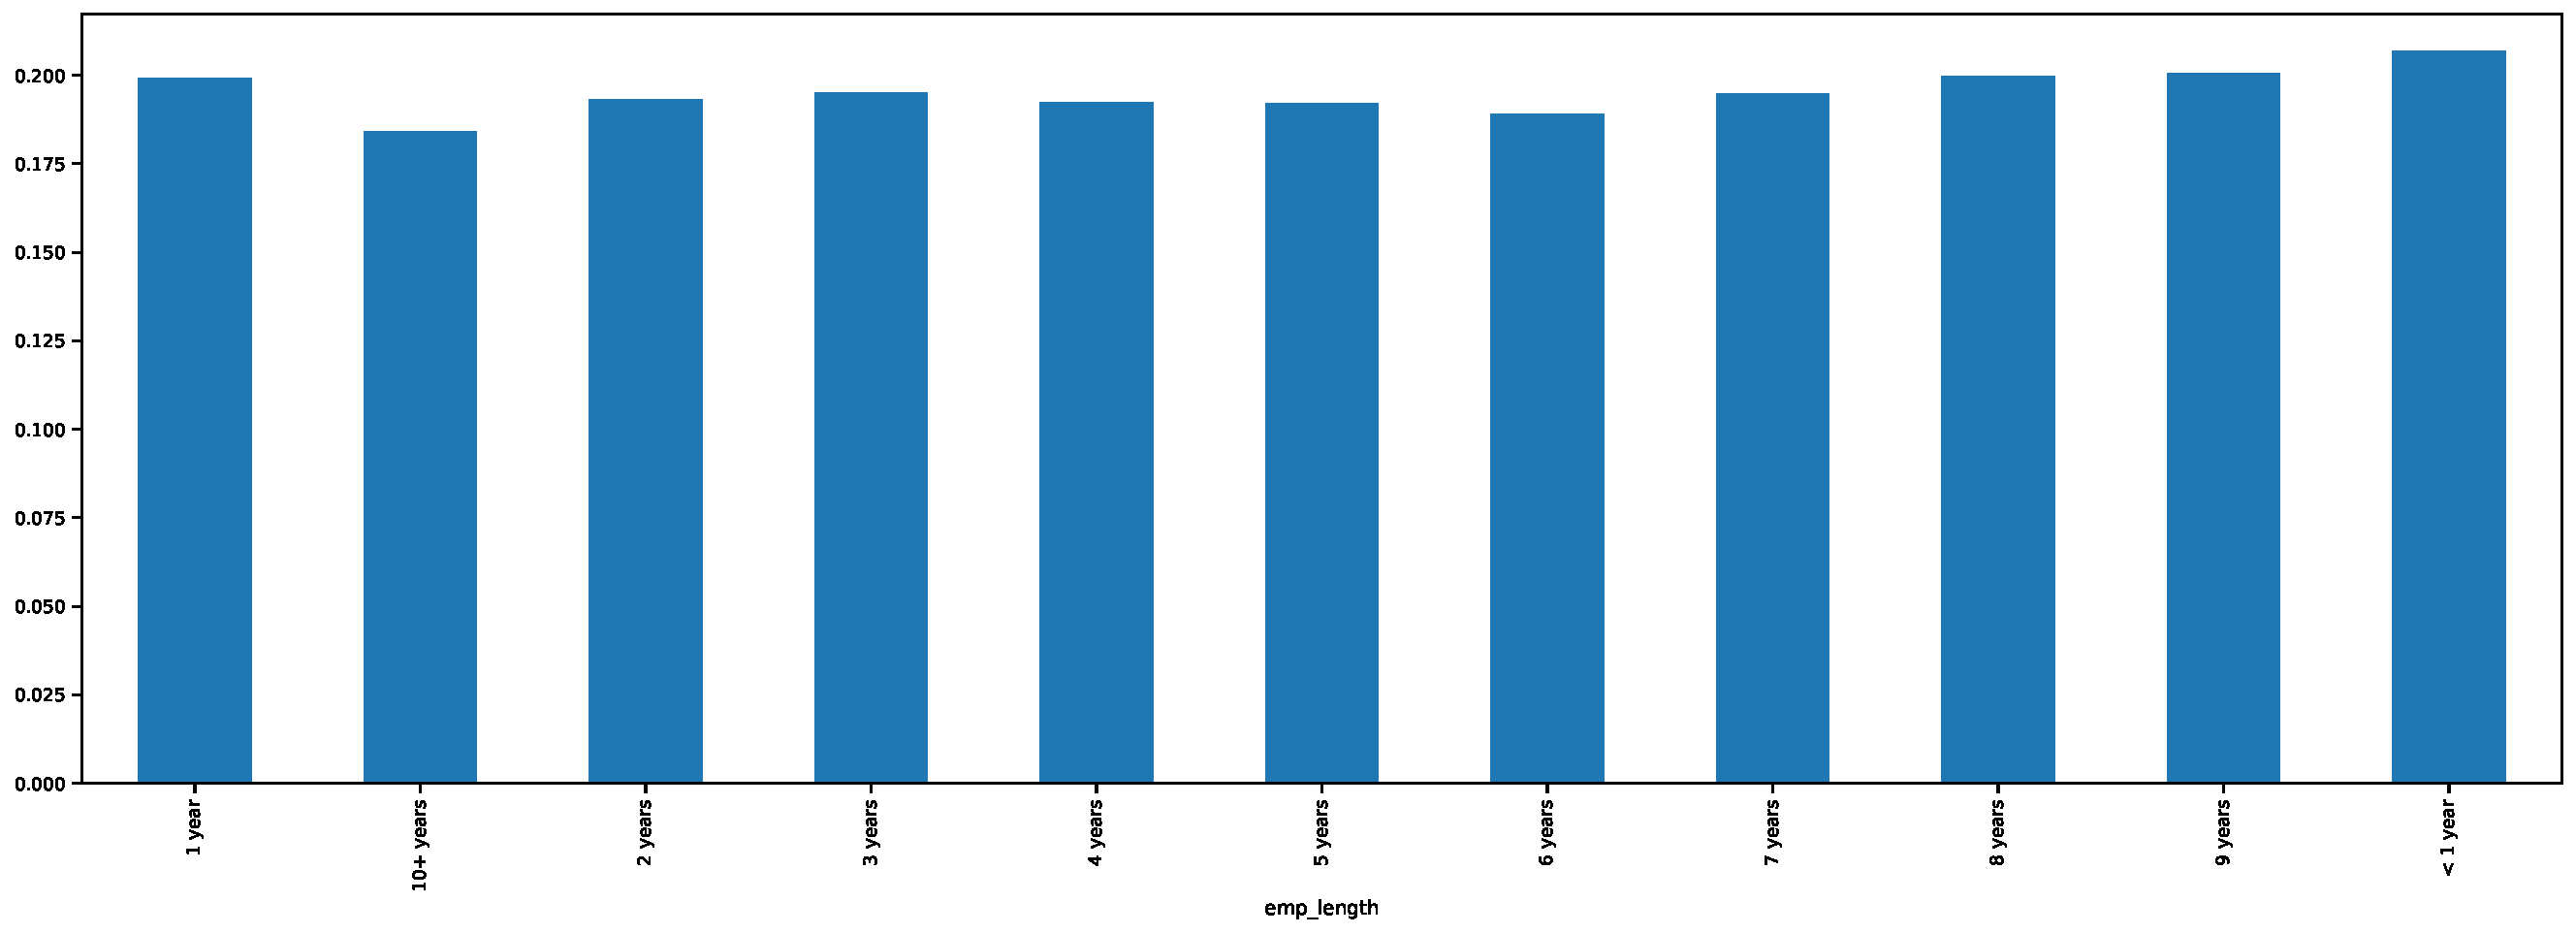
\includegraphics[scale=0.3]{figures/(4)emp_lenght_bar.pdf}
	\caption{barplot emp\_lenght\_bar distribution}
    \end{figure}
\section{Modelling [module: machine\_learning]}
We tried to use two different models, an algorithm such as XGBoost and a neural network model.\\
Regarding the optimization of these models, we saw as a first instance that the class to be predicted was highly unbalanced, with a ratio of 4:1.\\
We decided therefore to adopt a technique to rebalance the dataset called SMOTE (Synthetic Minority Oversampling).\\
This technique relies on resampling the data in such a way as to create new instances through k neighbors on imaginary lines connecting minority class values.
\subsection{X-G Boost}
As a first step, we built a preliminary model, instead of determining the best number of trees with cross validation we implemented a ’Early Stopping’ callback to stop training when the model doesn’t learn anymore.\\ 
To evaluate the XGBoost model we used AUC value. Once the first preliminary model is trained we have verified how well it works plotting a confusion matrix.\\
It can predict very well the majority class but not as well the minority.\\
For instance we tried to optimaze the hyperparameters also doing Cross Validation, with Grid Search.\\
	\begin{figure}[h!]
	\centering
	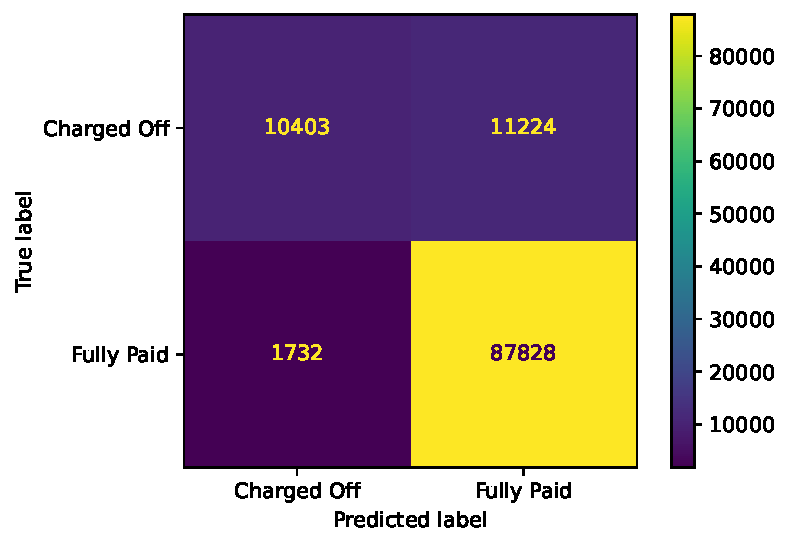
\includegraphics[scale=0.8]{figures/(5)basic_balanced_XGBoost.pdf}
	\caption{Confusion matrix XG-Boost without hyperparameters}
\end{figure}
	\begin{figure}[h!]
	\centering
	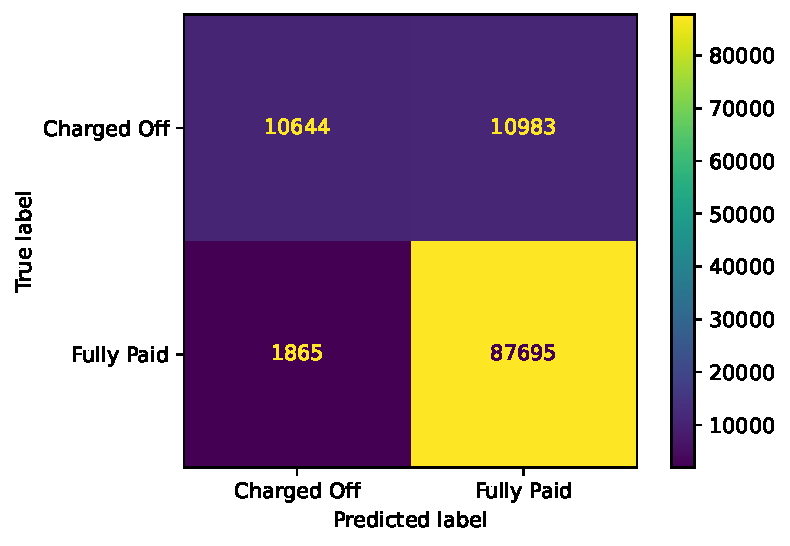
\includegraphics[scale=0.8]{figures/(6)hyper_balanced_XGBoost.pdf}
	\caption{Confusion matrix XG-Boost with hyperparameters}
\end{figure}
\subsection{Deep Neural Network}
For this model we proceed in several steps.\\
We built an “inverted pyramid” model and also here to avoid overfitting we used a validation set and we implemented a ’Early Stopping’ callback. \\
We added other layers using Dropout regolarization and compared the two models.\\
The regolarization gave us the best results so we procedeed always considering Dropout.\\
After this we tried to train another model called “diamond” and compare to the precedents one. \\
All the models we trained and tested give us results very similar but at the end the best one has been the “inverted pyramid” model with Dropout regolarization.\\
Also in this case we tried to optimize the hyperparamenters, doing Cross Validation, with Random Search. 
	\begin{figure}[h!]
	\centering
	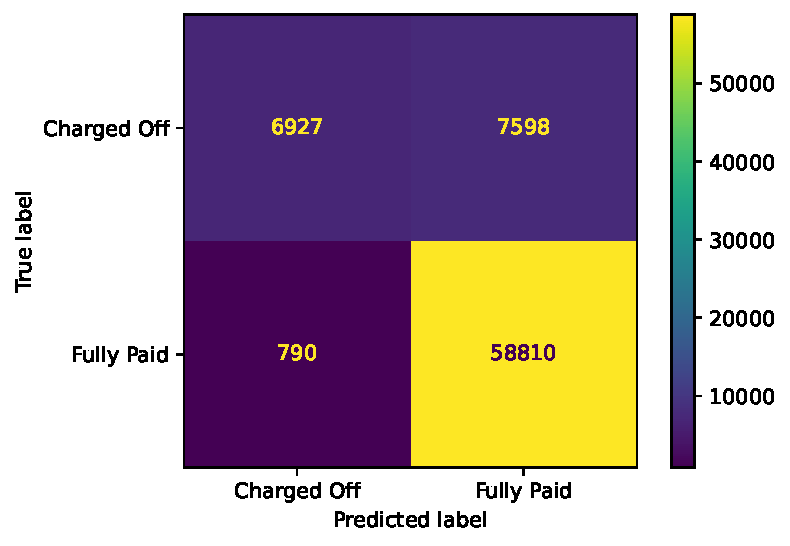
\includegraphics[scale=0.8]{figures/(7)confusion_matrix_basic_neural_network.pdf}
	\caption{Confusion matrix DNN without dropout}
\end{figure}
	\begin{figure}[h!]
	\centering
	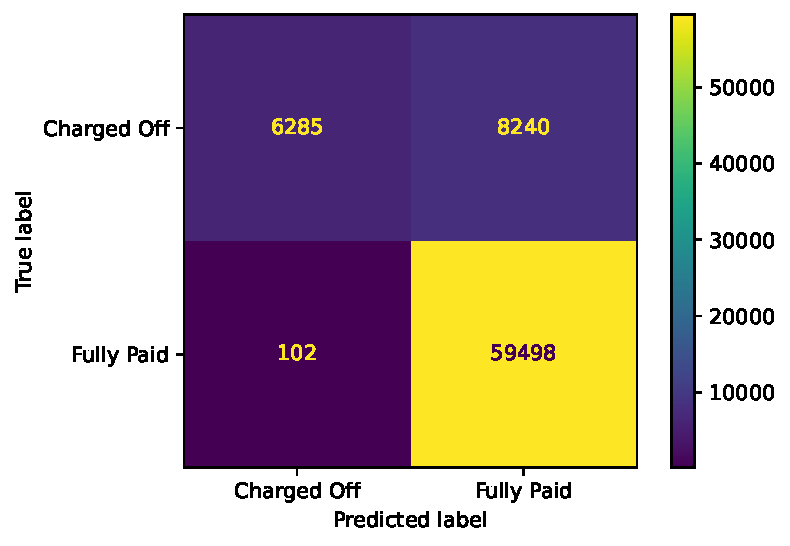
\includegraphics[scale=0.8]{figures/(8)confusion_matrix_dropout_neural_network.pdf}
    \caption{Confusion matrix DNN with dropout}
\end{figure}
	\begin{figure}[h!]
	\centering
	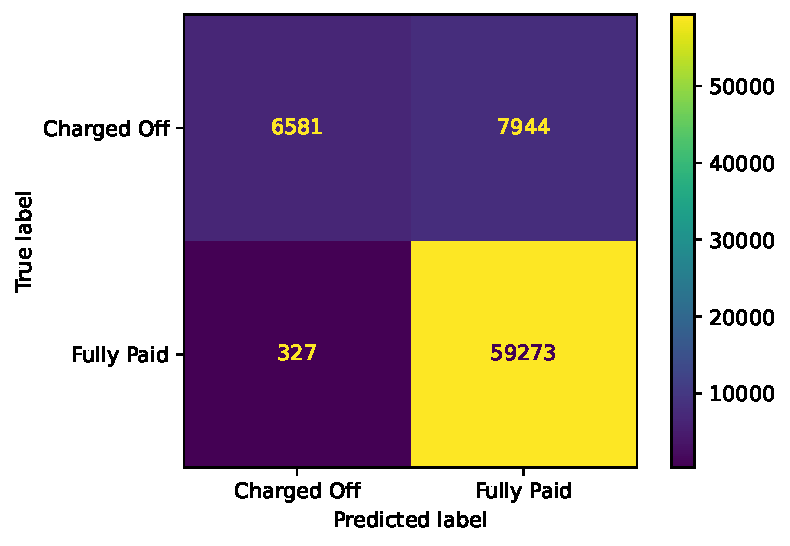
\includegraphics[scale=0.8]{figures/(9)confusion_matrix_dropout_diamond_neural_network.pdf}
	\caption{Confusion matrix diamond DNN with dropout}
\end{figure}
	\begin{figure}[h!]
	\centering
	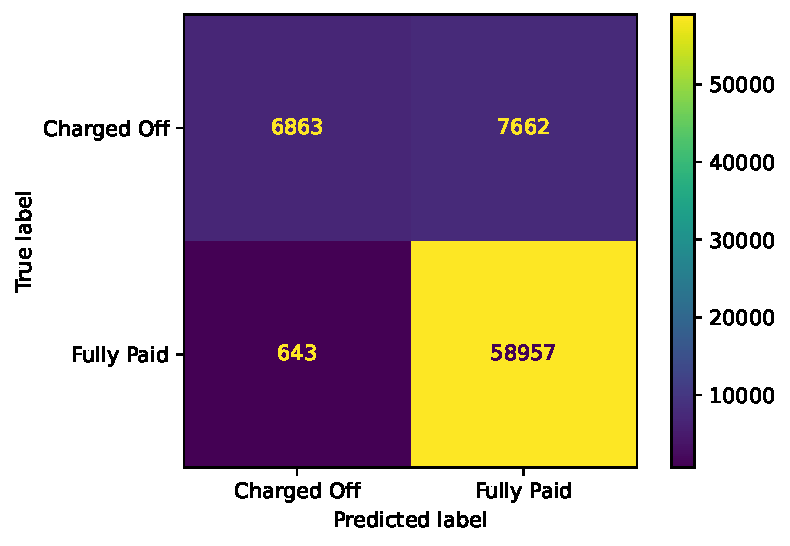
\includegraphics[scale=0.8]{figures/(10)confusion_matrix_hyper_neural_network.pdf}
	\caption{Confusion matrix DNN with hyperparameters}
\end{figure}
\section{Conclusion}
In this table we summarize the results of our model:
\[
\begin{array}{ccccc}
	\toprule
	\text{model} & \text{Accuracy} & \text{Precision} & \text{Recall} & \text{F1 Score}   \\
	\midrule
	\text{Basic XGBoost} & 0.8835 & 0.8867 & 0.9807 & 0.9313 \\
	\text{Hyperparameters XGBoost} & 0.8844 & 0.8887 & 0.979 & 0.9317 \\
	\text{Basic DNN} & 0.8543 & 0.9086 & 0.9104 & 0.9095 \\
	\text{Dropout DNN} & 0.8874 & 0.8783 & 0.9982 & 0.9344 \\
	\text{Diamond DNN} & 0.8544 & 0.9086 & 0.9104 & 0.9095 \\
	\text{Hyperprameter DNN} & 0.8880 & 0.8850 & 0.9892 & 0.9342 \\
	\bottomrule
\end{array}
\]
As we can see we have obtained great results in each metrics but f1 score.\\
On confusion matrix we have obtained a great prediction of the majority class $\sim$ 90 $\%$ in every model but a worse one on minority $\sim$ 54 $\%$.
This not so optimal classification is due to the beginning unbalanced of our dataset.\\
From our model, DNN predicts better than XGBoost.
\end{document}